%!TEX program = xelatex
%!LW recipe=latexmk (xelatex)
\documentclass[10pt]{article}

\usepackage{utils/styles}
\usepackage{utils/fonts}
\fontEstedadAsDefault
\fontComicSansMSAsLatin
\fontRecursiveMonoAsMono

% Define colors
\definecolor{blackbg}{RGB}{24, 24, 24}
\definecolor{accentgray}{RGB}{68, 84, 106}
\definecolor{accentlightgray}{RGB}{180, 186, 191}
%
\definecolor{accent}{RGB}{68, 114, 196}
\definecolor{accentlight}{RGB}{180, 199, 231}
\definecolor{accentbg}{RGB}{217, 226, 243}
\definecolor{accentdark}{RGB}{47, 84, 150}
\definecolor{accenttext}{RGB}{30, 54, 96}
%
\definecolor{accentgreen}{RGB}{83, 129, 53}
\definecolor{accentgreenbg}{RGB}{215, 228, 207}
\definecolor{accentgreentext}{RGB}{56, 87, 36}
%
\definecolor{accentyellow}{RGB}{255, 217, 102}
\definecolor{accentyellowbg}{RGB}{255, 242, 204}
\definecolor{accentyellowtext}{RGB}{153, 115, 0}
%
\definecolor{accentred}{RGB}{238, 69, 64}
\definecolor{accentredbg}{RGB}{251, 235, 232}
\definecolor{accentredtext}{RGB}{166, 28, 0}
%

\newcommand{\QuestionText}[1]{
    {\textmi{\textcolor{accentdark}{\large #1}}}
    \vspace{-0.3em}\par
}

% Define the command for questions
\newcounter{question}
\newcommand{\Question}{
    \pagebreak
    \vspace{1em}
    \stepcounter{question}
    \setcounter{subquestion}{0}
    \noindent{\large{\textbf{\textcolor{red}{سوال \RL{\wnalpha{\arabic{question}}}:}}}\hspace{0.2em}}
}

% Define the command for subquestions
\newcounter{subquestion}
\newcommand{\SubQuestion}{
    \stepcounter{subquestion}
    \vspace{1em}
    {
        \setlength{\parindent}{0.5em} 
        \large\textbf{\textcolor{accent}{\alph{subquestion})}}\hspace{0.1em}
    }
}

% Add border to every page
\addborder{black}{thick}{accent}{thin}

\renewcommand{\title}{\RL{تمرین سری هفتم}}
\renewcommand{\author}{\RL{امیرحسین محمدزاده}}
\newcommand{\authordescription}{\RL{شماره دانشجویی: ۴۰۲۱۰۶۴۳۴}}

% Define the header and footer style
\configHeader{accent}{\title}{\author}

\begin{document}

\begin{titlepage}
    \coverpageahmz{\title}{دی ماه 1403}{ساختار و زبان کامپیوتر}{جناب آقای دکتر اسدی}{اول 03-04}
        {
            \textbf{\author} \\
            \authordescription
        }
        {
			اینجا جای عکس است....
            % \mkshadow[accentlightgray]{0.05}{-0.05}{1}{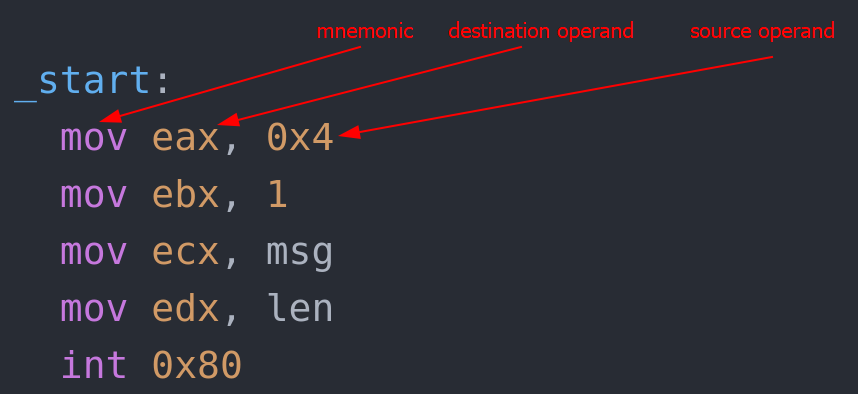
\includegraphics[width=0.7\textwidth]{files/main-image.png}}
            \\
            موضوع تمرین : \lr{x86 Assembly}
        }
\end{titlepage}

\newpage


\Question
\QuestionText{به سوالات  زیر پاسخ دهید:}

\QuestionText{به این‌جا بنگرید:}

\codeblockfile{c}{files/code.c}{style=xcode, bgcolor=accentbg,
%  lastline=20
 }{accentdark}{white}{}


    \SubQuestion
    \QuestionText{کد ماشین زیر را به اسمبلی برگردانید. فرض کنید اولین دستور در آدرس \texttt{0x00400000} است. می‌توانید از برچسب دلخواه استفاده کنید.}
    
    
    ببین من اومدم اینجا برای این کد زدم که بیاد بهمان کار رو بکنه....\\
    سلام بر تو 

    \SubQuestion
    \QuestionText{
    کد بالا چه کاری انجام می‌دهد؟ به ازای تمامی مقادیر ورودی بررسی کنید.
    }

    \SubQuestion
    \QuestionText{
    چه مشکلی در کد بالا وجود دارد؟ به ازای چه مقادیری اجرای کد پایان نمی‌یابد؟
    }

    \SubQuestion
    \QuestionText{برای رفع مشکل در کد بالا چه تغییری باید ایجاد کرد؟}
    
    سلام. این یک محتوای کد درون خطی است:
    \LR{\mintinline[bgcolor=blackbg, style=monokai]{c}{int main() { return 0; }}}

    سلام سلام خلاصه.


\Question
\QuestionText{به سوالات من جواب بدید:::}


    \SubQuestion
    \QuestionText{کد ماشین زیر را به اسمبلی برگردانید. فرض کنید اولین دستور در آدرس \texttt{0x00400000} است. می‌توانید از برچسب دلخواه استفاده کنید.}

    ببین من اومدم اینجا برای این کد زدم که بیاد بهمان کار رو بکنه....

    \SubQuestion
    \QuestionText{
    کد بالا چه کاری انجام می‌دهد؟ به ازای تمامی مقادیر ورودی بررسی کنید.
    }

    \SubQuestion
    \QuestionText{
    چه مشکلی در کد بالا وجود دارد؟ به ازای چه مقادیری اجرای کد پایان نمی‌یابد؟
    }

    \SubQuestion
    \QuestionText{برای رفع مشکل در کد بالا چه تغییری باید ایجاد کرد؟}
    
    سلام. این یک محتوای کد درون خطی است:
    \LR{\mintinline[bgcolor=blackbg, style=monokai]{c}{int main() { return 0; }}}

    سلام سلام خلاصه.

\end{document}
